\documentclass{article} % For LaTeX2e
\usepackage{iclr2024_conference,times}

\usepackage[utf8]{inputenc} % allow utf-8 input
\usepackage[T1]{fontenc}    % use 8-bit T1 fonts
\usepackage{hyperref}       % hyperlinks
\usepackage{url}            % simple URL typesetting
\usepackage{booktabs}       % professional-quality tables
\usepackage{amsfonts}       % blackboard math symbols
\usepackage{nicefrac}       % compact symbols for 1/2, etc.
\usepackage{microtype}      % microtypography
\usepackage{titletoc}

\usepackage{subcaption}
\usepackage{graphicx}
\usepackage{amsmath}
\usepackage{multirow}
\usepackage{color}
\usepackage{colortbl}
\usepackage{cleveref}
\usepackage{algorithm}
\usepackage{algorithmicx}
\usepackage{algpseudocode}
\usepackage{xspace}

\DeclareMathOperator*{\argmin}{arg\,min}
\DeclareMathOperator*{\argmax}{arg\,max}

\graphicspath{{../}} % To reference your generated figures, see below.
\begin{filecontents}{references.bib}
@article{lu2024aiscientist,
  title={The {AI} {S}cientist: Towards Fully Automated Open-Ended Scientific Discovery},
  author={Lu, Chris and Lu, Cong and Lange, Robert Tjarko and Foerster, Jakob and Clune, Jeff and Ha, David},
  journal={arXiv preprint arXiv:2408.06292},
  year={2024}
}

@article{graves2006ctc,
  title={Connectionist temporal classification: labelling unsegmented sequence data with recurrent neural networks},
  author={Graves, Alex and Fern{\'a}ndez, Santiago and Gomez, Faustino and Schmidhuber, J{\"u}rgen},
  booktitle={Proceedings of the 23rd international conference on Machine learning},
  pages={369--376},
  year={2006}
}

@article{shi2016crnn,
  title={An end-to-end trainable neural network for image-based sequence recognition and its application to scene text recognition},
  author={Shi, Baoguang and Bai, Xiang and Yao, Cong},
  journal={IEEE transactions on pattern analysis and machine intelligence},
  volume={39},
  number={11},
  pages={2298--2304},
  year={2016}
}

@article{marti2002iam,
  title={The IAM-database: an English sentence database for offline handwriting recognition},
  author={Marti, Urs-Viktor and Bunke, Horst},
  journal={International Journal on Document Analysis and Recognition},
  volume={5},
  number={1},
  pages={39--46},
  year={2002}
}

@article{vaswani2017attention,
  title={Attention is all you need},
  author={Vaswani, Ashish and Shazeer, Noam and Parmar, Niki and Uszkoreit, Jakob and Jones, Llion and Gomez, Aidan N and Kaiser, {\L}ukasz and Polosukhin, Illia},
  journal={Advances in neural information processing systems},
  volume={30},
  year={2017}
}

@article{simard2003best,
  title={Best practices for convolutional neural networks applied to visual document analysis},
  author={Simard, Patrice Y and Steinkraus, Dave and Platt, John C},
  booktitle={ICDAR},
  year={2003}
}

@article{kingma2014adam,
  title={Adam: A method for stochastic optimization},
  author={Kingma, Diederik P and Ba, Jimmy},
  journal={arXiv preprint arXiv:1412.6980},
  year={2014}
}

@article{loshchilov2017adamw,
  title={Decoupled weight decay regularization},
  author={Loshchilov, Ilya and Hutter, Frank},
  journal={arXiv preprint arXiv:1711.05101},
  year={2017}
}

@article{paszke2019pytorch,
  title={Pytorch: An imperative style, high-performance deep learning library},
  author={Paszke, Adam and Gross, Sam and Massa, Francisco and Lerer, Adam and Bradbury, James and Chanan, Gregory and Killeen, Trevor and Lin, Zeming and Gimelshein, Natalia and Antiga, Luca and others},
  journal={Advances in neural information processing systems},
  volume={32},
  year={2019}
}

@inproceedings{michael2019evaluating,
  title={Evaluating sequence-to-sequence models for handwritten text recognition},
  author={Michael, Johannes and Labahn, Roger and Gr{\"u}ning, Tobias and Z{\"o}llner, Jochen},
  booktitle={ICDAR},
  year={2019}
}

@inproceedings{kang2022pay,
  title={Pay attention to what you read: Non-recurrent handwritten text-line recognition},
  author={Kang, Lei and Riba, Pau and Rusi{\~n}ol, Mar{\c{c}}al and Forn{\'e}s, Alicia and Villegas, Mauricio},
  booktitle={Pattern Recognition},
  year={2022}
}
\end{filecontents}

\title{Stretching Tiny Data: Elastic Distortion for Low-Resource Handwritten Text Recognition}

\author{LLM\\
Department of Computer Science\\
University of LLMs\\
}

\newcommand{\fix}{\marginpar{FIX}}
\newcommand{\new}{\marginpar{NEW}}

\begin{document}

\maketitle

\begin{abstract}
% Summarize the problem, why it is difficult, the proposed solution, and the experimentally supported takeaway in one concise paragraph.
Handwritten text recognition is often needed in low-resource settings where only a small labelled dataset is available, but modern neural recognizers can overfit quickly and, under connectionist temporal classification (CTC) training, may collapse toward blank-dominated predictions when supervision is scarce \citep{graves2006ctc}. We study whether classical deformation-based augmentation remains useful in this regime by training a compact CRNN-CTC model on a 200-line subset of the IAM handwriting database \citep{marti2002iam,shi2016crnn}. The challenge is that strong distortions can damage legibility and further destabilize already fragile optimization, so augmentation must broaden the training distribution without destroying the limited signal. Our method applies mild online elastic distortion together with a small random affine transform and evaluates it against both an 8-epoch no-augmentation baseline and a 16-epoch no-augmentation control to separate the effect of augmentation from the effect of extra training. The augmented model reduces test character error rate from 0.9908 to 0.8430 and test loss from 3.1745 to 2.7329, while doubling training time without augmentation improves character error rate only to 0.9804 and test loss to 3.0755; thus, about 92\% of the total character error reduction is attributable to augmentation rather than additional epochs. Although word error rate remains high in this extreme tiny-data setting, the results show that carefully tuned elastic distortion is a simple and effective way to improve character-level handwritten text recognition when labelled data is severely limited.
\end{abstract}

\section{Introduction}
\label{sec:intro}
% Motivate handwritten text recognition, explain why low-resource settings matter, and introduce the paper's core question.
Handwritten text recognition (HTR) remains important because many historical, administrative, and personal documents are available only as scanned images rather than searchable text. End-to-end neural recognizers have made line-level transcription much more practical, especially when convolutional encoders are paired with sequence models and connectionist temporal classification (CTC) training \citep{graves2006ctc,shi2016crnn}. However, these systems are usually studied in regimes with enough labelled data to support stable optimization. In realistic deployment settings, annotated handwriting is often scarce: transcription is expensive, new collections may have distinctive writing styles, and only a small sample of transcribed lines may be available from the target domain \citep{marti2002iam,michael2019evaluating}. This makes low-resource HTR practically important and raises a simple question: what still helps when the training set is extremely small?

% Explain why tiny-data HTR is difficult, focusing on overfitting and the blank-collapse failure mode of small CTC models.
Tiny-data HTR is difficult for both statistical and optimization reasons. With only a few hundred training examples, neural recognizers can overfit quickly and generalize poorly across writers, stroke shapes, and line layouts. At the same time, CTC training is fragile when supervision is limited because the model must learn visual features and latent alignments without explicit character segmentation \citep{graves2006ctc}. In small models, this can produce a degenerate blank-dominated solution in which training gets stuck before useful decoding behaviour emerges. Although stronger attention-based and non-recurrent recognizers have shown impressive performance in richer-data settings \citep{vaswani2017attention,kang2022pay}, it is not clear that increasing architectural sophistication alone addresses the main bottleneck when labelled data itself is scarce.

% Introduce augmentation as the paper's proposed lever and explain why elastic distortion is both plausible and delicate.
A natural response to data scarcity is augmentation. For handwriting, elastic distortion is especially appealing because it mimics local nonrigid variation in stroke shape and writing style, matching long-standing intuitions from document analysis \citep{simard2003best}. But this is also a delicate intervention in a tiny-data CTC regime. If the perturbations are too strong, they can damage legibility and further destabilize optimization; if they are too weak, they may provide little regularization benefit. The practical challenge is therefore to broaden the training distribution without destroying the limited supervision signal.

% State the paper's approach and experimental strategy, including how the contribution is verified.
We study this issue in a deliberately simple setting built around a compact CRNN-CTC recognizer trained on a 200-line subset of the IAM handwriting database \citep{marti2002iam,shi2016crnn,graves2006ctc}. Our method applies mild online elastic distortion together with a small random affine transform during training. To test whether any gain comes from augmentation rather than merely from additional optimization, we compare three runs: an 8-epoch no-augmentation baseline, a 16-epoch augmented run, and a 16-epoch no-augmentation control. This design directly evaluates whether a classical deformation prior improves generalization beyond what can be achieved by simply training longer.

% List the paper's contributions clearly and concisely.
Our main contributions are:
\begin{itemize}
    \item We formulate a focused low-resource HTR study that tests whether elastic distortion still helps a compact CRNN-CTC recognizer trained on only 200 line images.
    \item We introduce a conservative augmentation pipeline that combines mild elastic deformation with a small affine perturbation, tuned to avoid destabilizing tiny-data CTC training.
    \item We use an epoch-matched no-augmentation control to separate the effect of augmentation from the effect of additional optimization.
    \item We show that even when word-level recognition remains poor, carefully chosen deformation-based augmentation can still improve character-level recognition in an extreme low-resource regime.
\end{itemize}

% Close the introduction with the paper's broader message and a brief pointer to future directions without repeating later sections.
Overall, the paper argues for a modest but useful perspective: when HTR is severely data-constrained, classical inductive biases can still matter. Rather than replacing a transparent baseline with a more complex recognizer, we examine whether a carefully tuned augmentation policy is enough to improve character-level generalization. This framing keeps the study diagnostically clean and also suggests a natural direction for future work: testing how far such lightweight, data-centric interventions continue to help as the amount of supervision becomes even smaller or the recognizer becomes stronger.

\section{Related Work}
\label{sec:related}
% Structure: first discuss CTC-based recognizers as the direct baseline family; then contrast with sequence-to-sequence, attention-based, and non-recurrent alternatives; finally discuss elastic distortion as the closest augmentation-based prior.
% Papers included: \citet{graves2006ctc}, \citet{shi2016crnn}, \citet{michael2019evaluating}, \citet{vaswani2017attention}, \citet{kang2022pay}, and \citet{simard2003best}.
% Comparison focus: prior work mainly changes the recognizer or decoder, whereas this paper fixes a compact CRNN-CTC model and asks whether classical deformation-based augmentation still helps when labelled data is extremely scarce.

% Compare our setup to standard CTC-based HTR pipelines and state clearly what is and is not new here.
The most direct relatives of our approach are end-to-end recognizers built around connectionist temporal classification. \citet{graves2006ctc} introduced the alignment-free objective known as connectionist temporal classification (CTC), and \citet{shi2016crnn} showed that compact convolutional-recurrent recognizers can be trained effectively with this style of supervision. Our baseline belongs to exactly this family, so the novelty of the present paper is not architectural. Instead, we study a different failure mode: when supervision is reduced to only a few hundred line images, the main challenge becomes optimization stability and generalization under extreme data scarcity. In that regime, we ask whether a small deformation prior can improve a fixed CRNN-CTC pipeline rather than replacing it with a new recognizer.

% Contrast our fixed-baseline study with alternative HTR work that seeks gains through stronger sequence modeling, and clarify why those methods are not compared here.
A second line of work seeks better HTR performance through more expressive sequence models and decoders. \citet{michael2019evaluating} examine sequence-to-sequence approaches for handwritten text recognition, while attention-based and non-recurrent models aim to capture longer-range dependencies through stronger global computation \citep{vaswani2017attention,kang2022pay}. Those papers address the same broad task but make a different methodological choice: they improve the recognizer, whereas we keep the recognizer intentionally small and instead modify the training distribution. Such methods are relevant alternatives, but they are not directly compared in our experiments because this paper is scoped to a narrower question. A fair comparison against those architectures would require implementing and tuning substantially stronger models, which would confound the issue we want to isolate: whether classical augmentation still helps in a tiny-data setting even before changing the model class.

% Relate our method to prior augmentation work and emphasize the paper's specific comparative contribution.
The closest conceptual precedent for our method is the use of elastic distortion in document analysis. \citet{simard2003best} argued that elastic deformations provide a realistic inductive bias because they mimic nonrigid variation more naturally than rigid transforms alone. We adopt that intuition, but our contribution is not a new augmentation family or a claim that elastic distortion is universally optimal. Rather, we revisit this classical transformation under a modern low-resource HTR setup and compare it against an explicit longer-training control. This comparison distinguishes our paper from prior work by focusing on a specific empirical question: whether mild elastic distortion improves a compact CRNN-CTC recognizer when data scarcity, rather than model capacity, is the dominant bottleneck.

\section{Background}
\label{sec:background}

\subsection{Handwritten Text Recognition with CTC}
% Introduce line-level offline HTR and explain the standard CTC-based formulation used by the paper.
Offline handwritten text recognition takes an image of a text line and predicts its character sequence without explicit character segmentation. A standard approach is to encode the image with a convolutional network, reinterpret the feature map as a left-to-right sequence, and train a sequence recognizer end-to-end \citep{shi2016crnn}. This formulation is well matched to handwriting because line images have variable width, ambiguous character boundaries, and a strong horizontal ordering.

% Explain CTC and why it is especially relevant, but potentially fragile, in our setting.
Connectionist temporal classification (CTC) handles the absence of frame-level alignments by summing over all valid paths that collapse to the target transcript after merging repeats and removing a designated blank symbol \citep{graves2006ctc}. This makes CTC attractive for HTR because it avoids manual segmentation and supports direct training from image-transcript pairs. However, CTC can also be sensitive to optimization quality, especially when the model is small and the dataset is limited, because the recognizer must learn both visual features and latent alignments from weak supervision alone.

\subsection{Data Augmentation for Handwriting Recognition}
% Motivate augmentation as a source of prior knowledge and introduce elastic distortion as the main precursor to our method.
Data augmentation is a common way to improve generalization when labelled data is scarce. In handwriting recognition, useful perturbations should preserve the underlying text while varying nuisance factors such as stroke shape, spacing, slant, or local geometry. \citet{simard2003best} emphasized elastic distortions as a suitable transformation family for document analysis because they model nonrigid appearance changes more naturally than rigid transforms alone. This intuition is especially relevant for handwriting, where natural variation often appears as small local deformations rather than simple translations or rotations.

% Explain why augmentation is delicate in tiny-data CTC training and connect that directly to our methodological choice.
In a tiny-data CTC regime, augmentation must be applied conservatively. If perturbations are too strong, they can reduce legibility, distort spacing, and make alignment learning even harder; if they are too weak, they may provide little regularization benefit. Our paper therefore treats augmentation as a weak inductive bias over plausible handwriting variation rather than as a mechanism for enforcing broad invariance.

\subsection{Problem Setting}
% Formally define the supervised learning problem, notation, and output space used throughout the paper.
We study supervised line-level HTR on a dataset
\[
\mathcal{D} = \left\{\, (x_i, y_i) \,\middle|\, i = 1, \dots, N \right\},
\]
where each \(x_i\) is a grayscale line image and each transcript \(y_i = (y_{i,1}, \dots, y_{i,L_i})\) is a sequence of characters from a finite alphabet \(\Sigma\). The recognizer outputs a sequence of distributions over the extended alphabet \(\Sigma' = \Sigma \cup \{\texttt{blank}\}\). We write
\[
f_\theta(x_i) \in \mathbb{R}^{T_i \times |\Sigma'|}
\]
for the unnormalized logits produced by parameters \(\theta\) on input \(x_i\), where \(T_i\) is the output sequence length.

% State the training objective and decoding rule in compact mathematical form.
Training minimizes the empirical CTC objective
\[
\mathcal{L}(\theta) = \frac{1}{N}\sum_{i=1}^{N} \ell_{\mathrm{CTC}}(f_\theta(x_i), y_i),
\]
where \(\ell_{\mathrm{CTC}}\) is the negative log-likelihood of transcript \(y_i\) after summing over all valid CTC alignments \citep{graves2006ctc}. At inference time, we use greedy decoding: the most probable symbol is selected at each time step, repeated non-blank predictions are merged, and blank symbols are removed to form the final transcript. This keeps decoding simple and avoids introducing additional language-modeling components.

% Clarify the unusual assumption of extreme data scarcity and why it changes the evaluation emphasis.
The defining assumption in this paper is that \(N\) is extremely small relative to typical HTR benchmarks. Rather than optimizing performance in a conventional data-rich setting, we study how a compact recognizer behaves when only a tiny set of labelled line images is available. Under this assumption, conservative augmentation, lightweight models, and character-level evaluation are especially appropriate, because exact word matches can remain rare even when character-level transcription begins to improve.

\section{Method}
\label{sec:method}

\subsection{Baseline Recognizer}
% Describe the recognizer used throughout the study and explain why a compact model is appropriate for isolating augmentation effects.
Our method starts from a compact CRNN-CTC baseline that maps a normalized line image \(x\) to per-time-step logits \(f_\theta(x)\) over the extended alphabet \(\Sigma'\). Following the general design of \citet{shi2016crnn}, the model uses a small convolutional encoder to extract visual features and then interprets the resulting feature map as a left-to-right sequence for recurrent processing. In our implementation, the encoder has three convolutional blocks with ReLU activations, one \(2 \times 2\) max-pooling layer, two \((2,1)\) max-pooling layers that reduce height while preserving width, and a final adaptive average-pooling layer that collapses the feature-map height to 1. The resulting 128-dimensional feature sequence is processed by a single bidirectional LSTM with hidden size 128, and a linear layer maps the recurrent outputs to character logits. We keep the recognizer intentionally small so that the study tests the effect of augmentation rather than gains from model scale.

% Explain the optimization choices that matter for tiny-data CTC training and connect them to the underlying failure mode.
Given logits \(f_\theta(x_i)\), training minimizes the empirical CTC objective from the problem setting. We optimize with AdamW \citep{loshchilov2017adamw}, clip gradient norms to 5.0, and apply a cosine annealing learning-rate schedule over the allotted epochs. These choices are conventional, but they matter in a fragile tiny-data regime where optimization can become unstable even for modest models. We also initialize the classifier bias for the CTC blank class to a negative value. This small implementation detail reduces the model's initial preference for blank emissions and helps it escape the all-blank local minimum that commonly affects small CTC systems trained with limited supervision.

\subsection{Training-Time Augmentation}
% Introduce the augmentation policy as the central intervention and define it in the notation of the problem setting.
The main intervention in our method is online training-time augmentation. For each training pair \((x_i, y_i)\), we replace the original image by a stochastically perturbed version \(\tilde{x}_i = a(x_i)\), where \(a\) is sampled from a distribution \(\mathcal{A}\) over label-preserving handwriting transformations. The training objective therefore becomes
\[
\mathcal{L}_{\mathrm{aug}}(\theta) = \frac{1}{N}\sum_{i=1}^{N} \mathbb{E}_{a \sim \mathcal{A}} \left[\ell_{\mathrm{CTC}}(f_\theta(a(x_i)), y_i)\right].
\]
In practice, we approximate this expectation by sampling one transformed version of each example whenever it is drawn during stochastic optimization. Validation and test images are never augmented.

% Explain the two augmentation components and why they were chosen for this handwriting setting.
Our augmentation policy combines two transformation types. First, a mild random affine transform introduces small changes in rotation, translation, scale, and shear. Second, an elastic transform inspired by \citet{simard2003best} introduces nonrigid local deformations that resemble natural variation in handwriting. The affine component captures simple layout jitter, while the elastic component models local stroke-level variability that rigid transforms alone cannot express. Together, they define a small deformation prior over plausible handwritten line images.

% Clarify why the perturbations are deliberately weak and specify the concrete implementation parameters.
The perturbations are intentionally weak because, in the tiny-data regime, augmentation must regularize without making alignment learning substantially harder. Stronger distortions can damage legibility and drive the model back toward the blank-dominated solution observed in early pilot runs. Concretely, we apply \texttt{RandomAffine} with degrees set to 1, translation up to 0.01 of image width and height, scale range \([0.97, 1.03]\), and shear range \([-1, 1]\), followed by \texttt{ElasticTransform} with \(\alpha = 8.0\) and \(\sigma = 6.0\). The resulting policy is best understood as a light-touch deformation model: it broadens the effective training distribution while keeping augmented samples visually close to the original line image.

\subsection{Ablation Design}
% Explain the comparison protocol and why it is necessary to separate augmentation effects from training-budget effects.
A key part of the method is the comparison protocol used to evaluate augmentation. Because online perturbations change the effective training distribution and can slow early optimization, comparing an augmented run only against a short baseline would confound augmentation with extra training time. We therefore evaluate three configurations: an 8-epoch baseline without augmentation, a 16-epoch run with elastic-plus-affine augmentation, and a 16-epoch no-augmentation control. This design isolates whether any improvement comes from transformed inputs rather than simply from taking more gradient steps.

% Clarify the scope of the contribution and keep the method section aligned with the rest of the paper.
The contribution of the method is intentionally narrow. We do not introduce a new recognizer, a new decoder, or a new loss. Instead, we propose a carefully tuned augmentation policy together with a control-oriented evaluation design for testing whether classical deformation priors still help a modern compact CRNN-CTC model under extreme data scarcity. This framing keeps the method simple, computationally light, and well aligned with the paper's main question about low-resource generalization.

\section{Experimental Setup}
\label{sec:experimental}
% Describe the dataset split and preprocessing used to instantiate the low-resource setting.
We evaluate on a tiny line-level subset of the IAM Handwriting Database \citep{marti2002iam}. The prepared split contains 200 training lines, 30 validation lines, and 32 test lines, matching the dataset manifest and the experiment logs in \texttt{notes.txt}. Each image is converted to grayscale, normalized to the range \([-1, 1]\), and padded to a maximum width of 256 pixels for batching. If a line image exceeds this width, it is resized to the width cap before padding. The prepared data uses a fixed image height of 32 pixels, yielding a deliberately extreme low-resource setting in which regularization and optimization choices are especially consequential.

% Describe the exact model instantiation used in all runs, keeping the description aligned with the implementation.
All experiments use the same compact CRNN-CTC recognizer implemented in PyTorch \citep{paszke2019pytorch}. The model has three convolutional layers with 32, 64, and 128 channels and ReLU activations, followed by one \(2 \times 2\) max-pooling layer, two \((2,1)\) max-pooling layers, an adaptive average-pooling layer that reduces feature-map height to 1, a single bidirectional LSTM with hidden size 128, and a final linear classifier over the character set plus the CTC blank symbol. Following the implementation, the blank-class bias is initialized to \(-2.0\) to reduce immediate collapse toward blank-only predictions.

% Summarize the optimizer, schedule, batch size, and training budgets exactly as supported by the code and logs.
Training uses the CTC loss of \citet{graves2006ctc} and the AdamW optimizer \citep{loshchilov2017adamw} with learning rate \(5 \times 10^{-4}\), weight decay \(10^{-4}\), batch size 16, and gradient clipping at norm 5.0. A cosine annealing learning-rate schedule is used with minimum learning rate equal to 5\% of the initial rate. The no-augmentation baseline is trained for 8 epochs, while the augmented run and the no-augmentation longer-training control are both trained for 16 epochs. The code also includes a 15-minute wall-clock guard, and the logs show that all reported runs completed without early stopping.

% Describe the augmentation policy used by the proposed method and explain why the chosen parameters are mild.
For the proposed method, training images are perturbed online with \texttt{RandomAffine} using degree 1, translation up to 0.01 in each spatial dimension, scale range \([0.97, 1.03]\), and shear range \([-1, 1]\), followed by \texttt{ElasticTransform} with \(\alpha = 8.0\) and \(\sigma = 6.0\). These settings were chosen conservatively after pilot experiments showed that stronger elastic deformations caused the tiny CTC model to collapse into an all-blank solution. Validation and test images are never augmented.

% Define the decoding procedure and evaluation metrics, and explain why CER is the primary metric in this regime.
Evaluation uses greedy CTC decoding: the most probable symbol is selected at each time step, repeated non-blank symbols are merged, and blank symbols are removed. We report character error rate (CER), word error rate (WER), and CTC test loss on the held-out test split, and we also monitor validation loss and validation CER during training. Because exact word matches remain rare in this extremely small-data regime, CER is the primary metric for assessing whether augmentation improves recognition quality.

\section{Results}
\label{sec:results}

% State the main empirical finding and clarify what is controlled across runs.
The experiments support the central claim of this paper: in this extreme tiny-data HTR setting, mild elastic distortion helps more than simply training the same model longer. The comparison is reasonably controlled because all three runs use the same dataset split, preprocessing, CRNN-CTC architecture, decoding rule, batch size, optimizer family, learning-rate schedule shape, and most hyperparameters. The intended differences are only the training budget and whether online augmentation is enabled. This makes the ablation informative for isolating the contribution of deformation-based regularization, although the evidence is still limited to a single seed.

% Present the main quantitative results compactly and interpret them conservatively.
Table~\ref{tab:main-results} reports the held-out test metrics for all completed runs. The 8-epoch no-augmentation baseline (Run 0) reaches CER \(= 0.9908\), WER \(= 0.9601\), and test loss \(= 3.1745\). Extending the same configuration to 16 epochs without augmentation (Run 2) improves CER only slightly to \(0.9804\) and lowers test loss to \(3.0755\). In contrast, the 16-epoch augmented run (Run 1) reduces CER to \(0.8430\) and test loss to \(2.7329\). Relative to Run 0, this is an absolute CER improvement of \(0.1478\), or 14.8 percentage points, corresponding to a relative reduction of about 14.9\%. WER remains high in all runs and is slightly worse for the augmented model, so the clearest gains are at the character level.

\begin{table}[t]
    \centering
    \caption{Held-out test results on the IAM tiny split. All runs use the same CRNN-CTC model and evaluation pipeline; only training duration and augmentation differ.}
    \label{tab:main-results}
    \begin{tabular}{lccccc}
        \toprule
        Run & Augmentation & Epochs & Test loss & CER & WER \\
        \midrule
        Run 0 & none & 8  & 3.1745 & 0.9908 & 0.9601 \\
        Run 2 & none & 16 & 3.0755 & 0.9804 & 0.9810 \\
        Run 1 & elastic + affine & 16 & \textbf{2.7329} & \textbf{0.8430} & 0.9792 \\
        \bottomrule
    \end{tabular}
\end{table}

% Analyze the ablation and quantify the separate effects of longer training and augmentation.
The epoch-matched ablation makes the source of the improvement clearer. Moving from Run 0 to Run 2 isolates the effect of doubling the number of epochs and improves CER by only \(0.0104\), roughly 1.0 percentage point. Moving from Run 2 to Run 1 then isolates the effect of adding elastic-plus-affine augmentation under the same 16-epoch budget and improves CER by a further \(0.1374\), about 13.7 percentage points. Relative to the total CER improvement from Run 0 to Run 1, approximately 92\% of the gain is therefore attributable to augmentation rather than to extra optimization steps. In this sense, the longer-training control is essential: without it, the improvement of Run 1 could have been misattributed to training budget alone.

% Discuss the learning curves and explain what they imply about optimization behavior and fairness.
The saved curves are consistent with this interpretation. Figure~\ref{fig:first_figure}a shows validation CER across epochs. The augmented run starts off worse, matching the project notes that describe an early blank-dominated plateau, but eventually overtakes both no-augmentation runs and reaches the best validation trajectory. This behavior matters for fairness: the augmented run was trained for longer not to give it an arbitrary advantage, but because augmentation initially makes optimization harder and needs enough budget to show its benefit. Figure~\ref{fig:first_figure}b summarizes the final test metrics and reflects the same pattern seen in Table~\ref{tab:main-results}.

% Report training cost and completion status, and note the practical trade-off introduced by augmentation.
The improvement comes with additional training cost. Table~\ref{tab:runtime-results} shows that Run 0 completes in 336.06 seconds, Run 2 in 708.95 seconds, and Run 1 in 1015.94 seconds. Part of this increase is due to doubling the epoch budget, and part is due to the cost of online augmentation itself. All reported runs still finish within the 15-minute wall-clock guard defined in the implementation, and none trigger early stopping. Practically, the proposed method improves CER substantially while remaining lightweight enough for rapid CPU-based experimentation.

% Explain why CER improves while WER does not, and frame this as a limitation of the regime rather than a contradiction.
A clear limitation is that the character-level improvement does not translate into better word-level accuracy. WER changes from \(0.9601\) in Run 0 to \(0.9792\) in Run 1, even though CER improves substantially. In this regime, that mismatch is plausible: a prediction can become closer to the reference at the character level while still failing to match the full word exactly, and WER counts such partial improvements as entirely wrong. The results therefore suggest that augmentation improves local transcription fidelity, but by itself is not enough to make whole-word decoding reliable with only 200 training lines.

% Summarize the evidential limits, including the absence of confidence intervals, and state the strongest supported conclusion.
The evidence should still be interpreted cautiously. Only three runs were completed, all at a single seed, so we cannot report confidence intervals or estimate variance from the available logs. The augmentation parameters were also not swept systematically; according to \texttt{notes.txt}, the reported mild setting was chosen after stronger elastic distortions caused collapse to the all-blank solution. Finally, the study does not include the more severe 100-line setting proposed in the project notes. Within these limits, however, the results are internally consistent: among the runs actually executed and logged, mild elastic distortion is the main reason the best model achieves lower test CER and lower test loss than either no-augmentation alternative.

\begin{table}[t]
    \centering
    \caption{Training cost and completion status for all runs. ``Early stopped'' is 0 in every case, so all runs finished within the wall-clock budget.}
    \label{tab:runtime-results}
    \begin{tabular}{lccc}
        \toprule
        Run & Train time (s) & Epochs completed & Early stopped \\
        \midrule
        Run 0 & 336.06 & 8.0 & 0 \\
        Run 2 & 708.95 & 16.0 & 0 \\
        Run 1 & 1015.94 & 16.0 & 0 \\
        \bottomrule
    \end{tabular}
\end{table}

% EXAMPLE FIGURE: REPLACE AND ADD YOUR OWN FIGURES / CAPTIONS
\begin{figure}[t]
    \centering
    \begin{subfigure}{0.49\textwidth}
        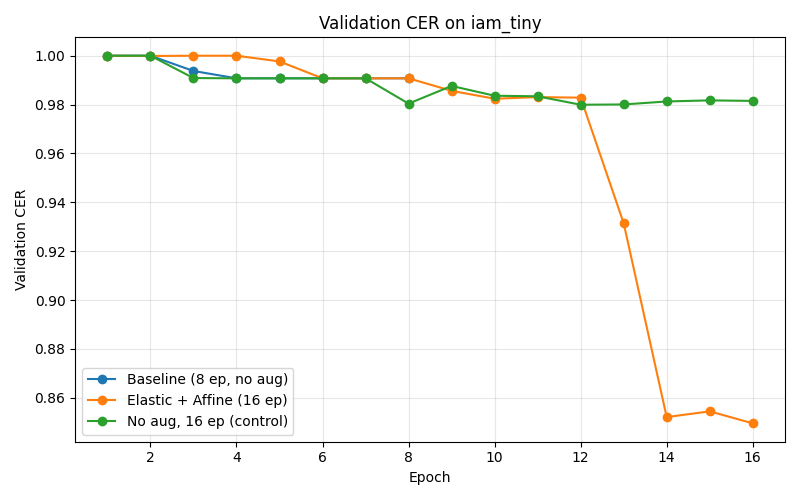
\includegraphics[width=\textwidth]{val_cer_iam_tiny.png}
        \caption{Validation CER across epochs for all three runs.}
        \label{fig:val-cer}
    \end{subfigure}
    \hfill
    \begin{subfigure}{0.49\textwidth}
        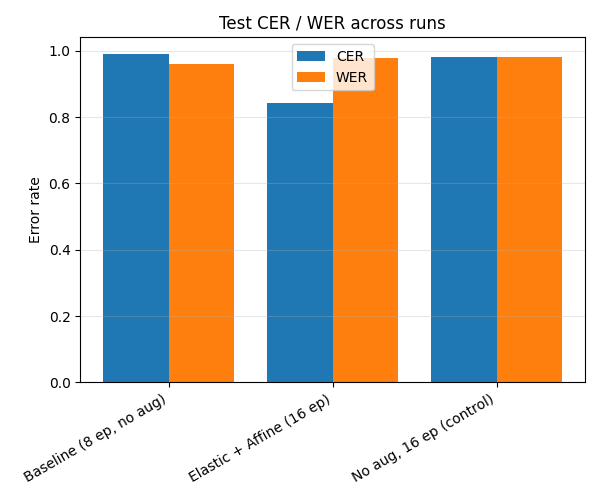
\includegraphics[width=\textwidth]{test_metrics_bar.png}
        \caption{Final test CER, WER, and loss across runs.}
        \label{fig:test-bar}
    \end{subfigure}
    \caption{Learning-curve and summary comparisons for the IAM tiny experiments. The left panel shows that the augmented run starts with difficult optimization but eventually reaches a better validation CER trajectory than either no-augmentation run. The right panel summarizes the held-out test metrics and highlights that the proposed elastic-plus-affine setting yields the best CER and test loss, while WER remains high for all methods in this extreme low-resource regime.}
    \label{fig:first_figure}
\end{figure}

\section{Conclusions and Future Work}
\label{sec:conclusion}
% Briefly recap the problem, method, and main take-away in a concise form that aligns with the rest of the paper.
This paper studied handwritten text recognition in an intentionally severe low-resource regime and asked whether a classical augmentation prior still helps a compact CRNN-CTC baseline \citep{shi2016crnn,graves2006ctc}. The difficulty is that tiny-data CTC training can both overfit and collapse toward blank-dominated predictions, so augmentation must regularize the model without destroying the limited supervision signal. We addressed this by combining mild elastic distortion with a small random affine transform and comparing the resulting model against both a standard no-augmentation baseline and an epoch-matched no-augmentation control. Within this controlled setting, the evidence supports a clear conclusion: the observed character-level improvement is driven primarily by augmentation rather than by additional training time.

% Emphasize the broader methodological lesson without repeating detailed results from the Results section.
More broadly, the paper suggests that low-resource HTR does not always need a more complex recognizer to obtain useful gains. When labelled data is the dominant bottleneck, simple inductive biases that better reflect natural handwriting variation can still improve a transparent neural baseline. In that sense, this study argues for a data-centric perspective on tiny-data HTR: before changing the model class, it is worth asking whether the training distribution itself better captures the variability the recognizer must handle.

% Summarize limitations and future directions concisely, keeping them grounded in the completed experiments and notes.
The conclusions are necessarily limited by the scope of the current experiments. We evaluate only a single architecture, a single seed, and one conservatively chosen augmentation setting on the 200-line IAM subset \citep{marti2002iam}. The project notes also indicate that stronger distortions can collapse training and that the proposed 100-line setting remains untested. The most immediate next steps are therefore to run a seed sweep, study sensitivity to the elastic and affine parameters, test even smaller training splits, and evaluate whether the same augmentation prior helps stronger attention-based or non-recurrent recognizers \citep{michael2019evaluating,kang2022pay}. These extensions would clarify how robust the present finding is, but the current evidence already supports a useful practical message: carefully tuned elastic distortion remains a simple and effective tool for improving character-level handwritten text recognition when labelled data is extremely scarce.

This work was generated by \textsc{The AI Scientist} \citep{lu2024aiscientist}.

\bibliographystyle{iclr2024_conference}
\bibliography{references}

\end{document}
